\begin{tcolorbox}[colback=white,colframe=black,opacityframe=0,colbacktitle=black,title={\textbf{Problem 6 [\examproblemweight\ points]}}]
Let $y=f(x)$ be the function defined by $2y+3x=12$.
\begin{enumerate}[label=(\alph*)]
	\item \textbf{(2 points)} Find the intercepts of the function $f$.
	\item \textbf{(2 points)} Determine the slope of $f$.
	\item \textbf{(4 points)} Based on the previous two parts, rewrite $y=f(x)$ in slope-intercept form and graph the function $f$ in the Cartesian plane below. (Though, it's okay if you already rewrote $y=f(x)$ in slope-intercept form to answer any of the previous two parts; just make sure it's correct, as your work for both the intercepts and slope will doubly-count for both parts.)\\
	\hspace*{17em}
	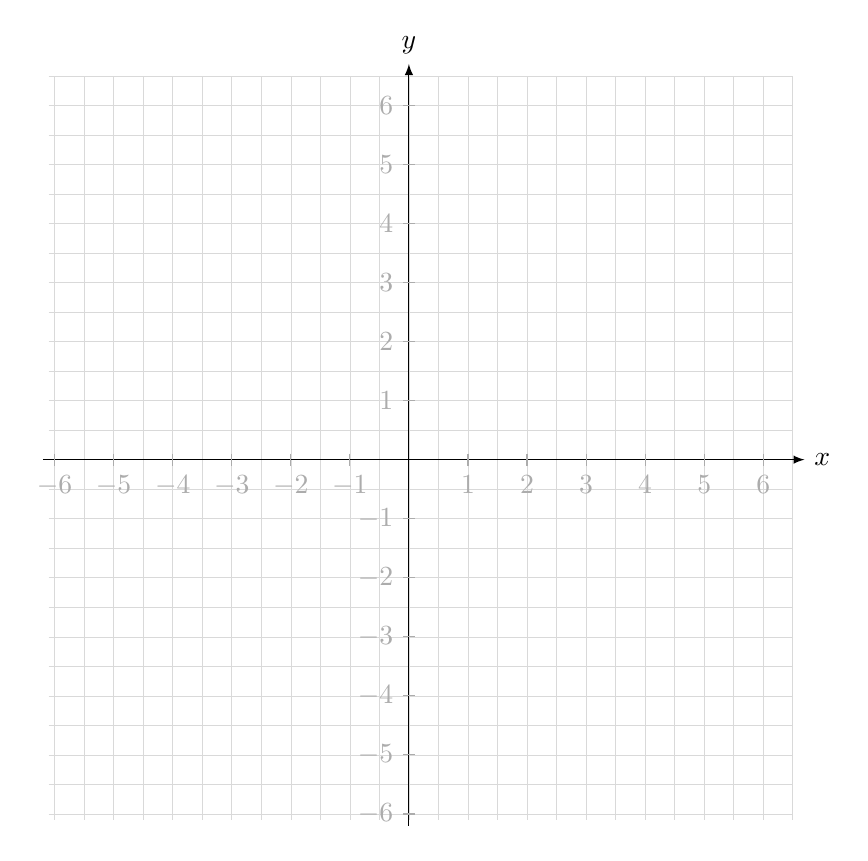
\begin{tikzpicture}[scale=0.75]
		\draw[very thin,color=black!15,step=.5] (-6.1,-6.1) grid (6.5,6.5);
		\draw[-latex] (-6.2,0) -- (6.7,0) node[right] {$x$};
		\draw[-latex] (0,-6.2) -- (0,6.7) node[above] {$y$};
		\foreach \i in {-6,...,-2,-1,1,2,...,6}
		\draw[gray!65] (\i,.1)--(\i,-.1) node[below] {$\i$};
		\foreach \i in {-6,...,-2,-1,1,2,...,6}
		\draw[gray!65] (.1,\i)--(-.1,\i) node[left] {$\i$};
	\end{tikzpicture}
	\item \textbf{(2 points)} Having found out what $f(x)$ is from the previous part, we observe that it is one-to-one. Determine its inverse $f^{-1}(x)$.
\end{enumerate}
\end{tcolorbox}

\newpage
\noindent \centering Blank page \thepage~for additional work
\newpage
